\documentclass[conference]{IEEEtran}

\usepackage[cmex10]{amsmath}
\usepackage{amssymb}

\usepackage{graphicx}
\usepackage{epstopdf}
\DeclareGraphicsExtensions{.eps,.pdf,.jpeg,.png}

\usepackage{abbrevs}
\newabbrev\SSPARC{Shared spectrum access between radar and communications (SSPARC)}[SSPARC]
\newabbrev\PAR{peak to average power (PAR)}[PAR]

\hyphenation{op-tical net-works semi-conduc-tor}

\begin{document}

\title{Some title}

\author{\IEEEauthorblockN{Joseph H. Kim and Robert Baxley}
\IEEEauthorblockA{Georgia Tech Research Institute,
Atlanta, Georgia 30318\\
Email: joseph.kim@gtri.gatech.edu, bob.baxley@gtri.gatech.edu}}
\maketitle

\begin{abstract}
This paper is .
\end{abstract}

\section{Introduction}
This demo file is intended to serve as a ``starter file''
for IEEE conference papers produced under \LaTeX\ using
IEEEtran.cls version 1.7 and later.

\subsection{Subsection Heading Here}
Subsection text here.


\subsubsection{Subsubsection Heading Here}
Subsubsection text here.


\section{Radar Spreading}
\SSPARC requires the mitigation of radar interference. One approach of this is to orthogonalize the communication and the radar signal.  Spectral spreading the communication signal ${\mathbf{x}\in \mathbb{C}^{N_x}}$ with the radar signal $\mathbf{r}\in \mathbb{C}^{N_r}$ is one way to approximate this orthogonalization.  The spread transmitted signal will be
\begin{equation}
\mathbf{y}=\mathbf{F}_r \mathbf{x}\\
\label{eq1}
\end{equation}  
where $\mathbf{x}$ is the communication constellation symbols, $\mathbf{F}_r$ is the convolution matrix of the radar signal.  To maintain the proper size of the signal, $N_x\geq N_r$, and $\mathbf{F}_r$ is a circular convolution with zero padding of$N_x-N_r$ to be $N_x\times N_x$ matrix.

The receiver will receive the signal
\begin{equation}
\mathbf{z}=\mathbf{F}_h \mathbf{F}_r \mathbf{x} +\beta[\mathbf{r},0,0,\dots,0,0]^T +\mathbf{n}\\
\label{eq2}
\end{equation} 
where $\mathbf{F}_h$ is the channel effect, The radar signal $\mathbf{r}$ is zero padded to match the size of the communication signal.

The pulse compression waveform of the radar signal allows for the following proprieties:
\begin{equation}
\mathbf{F}_r^H \mathbf{r} = [1,0,0,\dots,0,0]^T\approx\mathbf{0} \\
\label{prop1}
\end{equation}
\begin{equation}
\mathbf{F}_r^H \mathbf{F}_r \approx \mathbf{I}
\label{prop2}
\end{equation}
$H$ denotes the Hermitian conjugate of matrix and $T$ denote the Transpose of the matrix.
The de-spreading of the signal is done by
\begin{equation}
\mathbf{\hat{x}}=\mathbf{F}^H\mathbf{z}
\end{equation}
using the radar proprieties from \eqref{prop1} and \eqref{prop2} you get
\begin{equation}
=\mathbf{F}_h\mathbf{x}+\boldsymbol{\beta}[h,0,0,\dots,0,0]^T+\mathbf{F}^H\mathbf{n}
\end{equation} 

This shows that radar signal $\boldsymbol{\beta}$ has compressed, mitigating the interference to just few samples.  However there is a problem with this mitigation.  The \PAR of the signal is very high.  

The high \PAR causes nonlinear distortion when the signals come close to or exceeds the saturation level of the power amplifier.  To resolve this problem, several options were considered and analyzed.

\section{PAR Reduction}
The \PAR of the signal is defined as
\begin{equation}
PAR(x)=\frac{\Vert x \Vert^2_\infty}{\Vert x \Vert^2_2/N_x}
\end{equation}
where $\Vert\cdot\Vert_l$ denotes the $l$-norm of the vector.  Since radar spreading aggregate the signal to $y_i=\sum_{j=0}^{N_x-1} {F_r}_{ij}x_j$ , and since $x$ is i.i.d random variable with expectation $E[x_j]=\mu$ and variance $Var[x_i]=\sigma^2$.  This means that signal $y$ has expectation $E[\mathbf{y}]\approx N_x\mu$ and variance $Var[\mathbf{y}\approx N_x\sigma^2$.  As a result, the radar spread signal tends to have high \PAR.

Having a high \PAR means that the signal power inefficient and is prone to non-linear distortion from power amplifier.  A general \PAR reduction problem for aggregated signal is given by 
\begin{equation}
     \begin{aligned}
      &\text{Minimize } & &\left\Vert\sum_{p=1}^P\alpha_pA_p\left(x_p^{(k)}+\epsilon_p^{(k)}\right)\right\Vert_\infty  \\
      &\text{Subject to} &  &k\in \mathcal{K} \\
      & & &\alpha_p\in\mathcal{A}_p\\
      & & &\epsilon_p^{(k)}\in\mathcal{E}_p 
     \end{aligned}
\end{equation}

where $\mathcal{K}$ is a set of alternate signal, $\mathcal{A}$ is a set of combination value, and $\mathcal{E}$ is a set of allowed error values.  Since the combination value have very limited effect on the \PAR reduction, we will focus on the alternate signals and error values.
\subsection{Alternate signals}
the transmitted signal \eqref{eq1} can be expanded as
\begin{gather*}
y^{(1)}=F_rx_1^{(1)}+F_rx_2^{(1)}+F_rx_3^{(1)}+\cdots \\
y^{(2)}=F_rx_1^{(2)}+F_rx_2^{(2)}+F_rx_3^{(2)}+\cdots \\
\vdots \\
y^{(\mathcal{K})}=F_rx_1^{(\mathcal{K})}+F_rx_2^{(\mathcal{K})}+F_rx_3^{(\mathcal{K})}+\cdots
\end{gather*}
where $\mathcal{K}$ number of alternate way to represent same communication information or get the same radar knowledge and the receiver is aware of all the alternative possibility and determine which method was used.  We may be able to reduce \PAR by selecting a method that gives a signal with the lowest \PAR.  
\begin{figure}
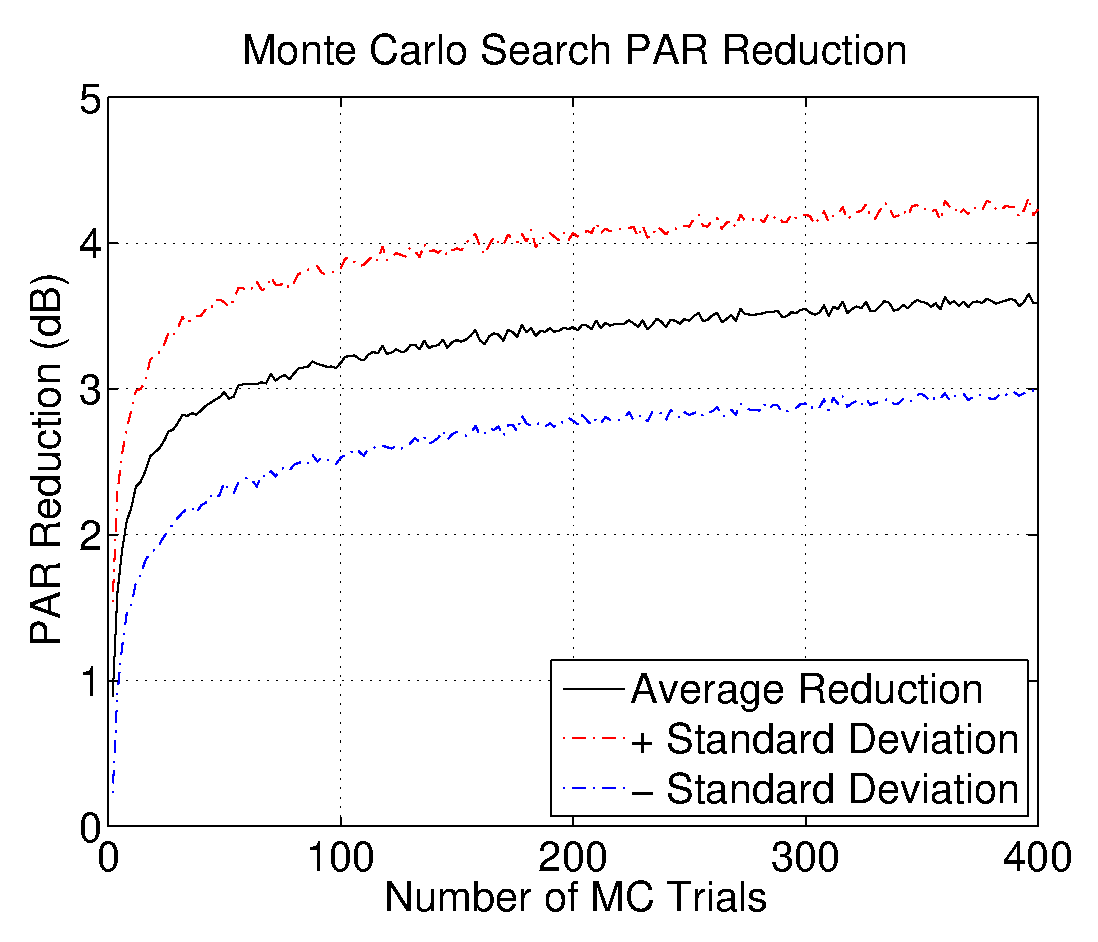
\includegraphics[width=\linewidth]{MCFig.eps}
\caption{Monte Cario search of alternate signals}
\end{figure}

\begin{thebibliography}{1}

\bibitem{IEEEhowto:kopka}
H.~Kopka and P.~W. Daly, \emph{A Guide to \LaTeX}, 3rd~ed.\hskip 1em plus
  0.5em minus 0.4em\relax Harlow, England: Addison-Wesley, 1999.

\end{thebibliography}




% that's all folks
\end{document}
